\chapter{Metode dan Kurva Titrasi}\label{ch:b1:titration-methods}

Seorang apoteker menerima sejumlah tablet vitamin C berlabel
\qty{500}{mg} dan, sebelum tablet-tablet itu dijual, harus memastikan
bahwa setiap tablet memuat jumlah yang tertera pada label. Ia tidak akan
menimbang vitaminnya secara langsung: vitamin itu tercampur dengan bahan
pengikat dan bahan pengisi. Ia akan mentitrasinya --- mereaksikannya
dengan pereaksi yang konsentrasinya diketahui, mengukur volume yang
diperlukan, lalu menghitung jumlahnya. Reaksi apa, bagaimana melihat
akhirnya, dan seberapa yakin hasilnya: itulah pertanyaan-pertanyaan bab
ini, yang membawa kesetimbangan-kesetimbangan lima bab terakhir ke meja
laboratorium.

\begin{recall}
Jilid sekolah (kelas 11 dan 12) mentitrasi asam dengan basa melalui
perubahan warna, mengikuti \omterm{def:b1:titration-methods:titration}{titrasi} dengan pH meter dan konduktometer,
dan memakai hubungan \omterm{def:b1:titration-methods:titration}{ekuivalensi} $C_AV_A = C_BV_B$. Metode \omterm{def:b1:predominant-reaction:predominant-reaction}{reaksi
predominan} terdapat pada \cref{ch:b1:predominant-reaction};
kesetimbangan pengendapan, kompleksasi, dan redoks pada
\cref{ch:b1:precipitation,ch:b1:complexation,ch:b1:nernst}.
\end{recall}

\begin{omfigure}
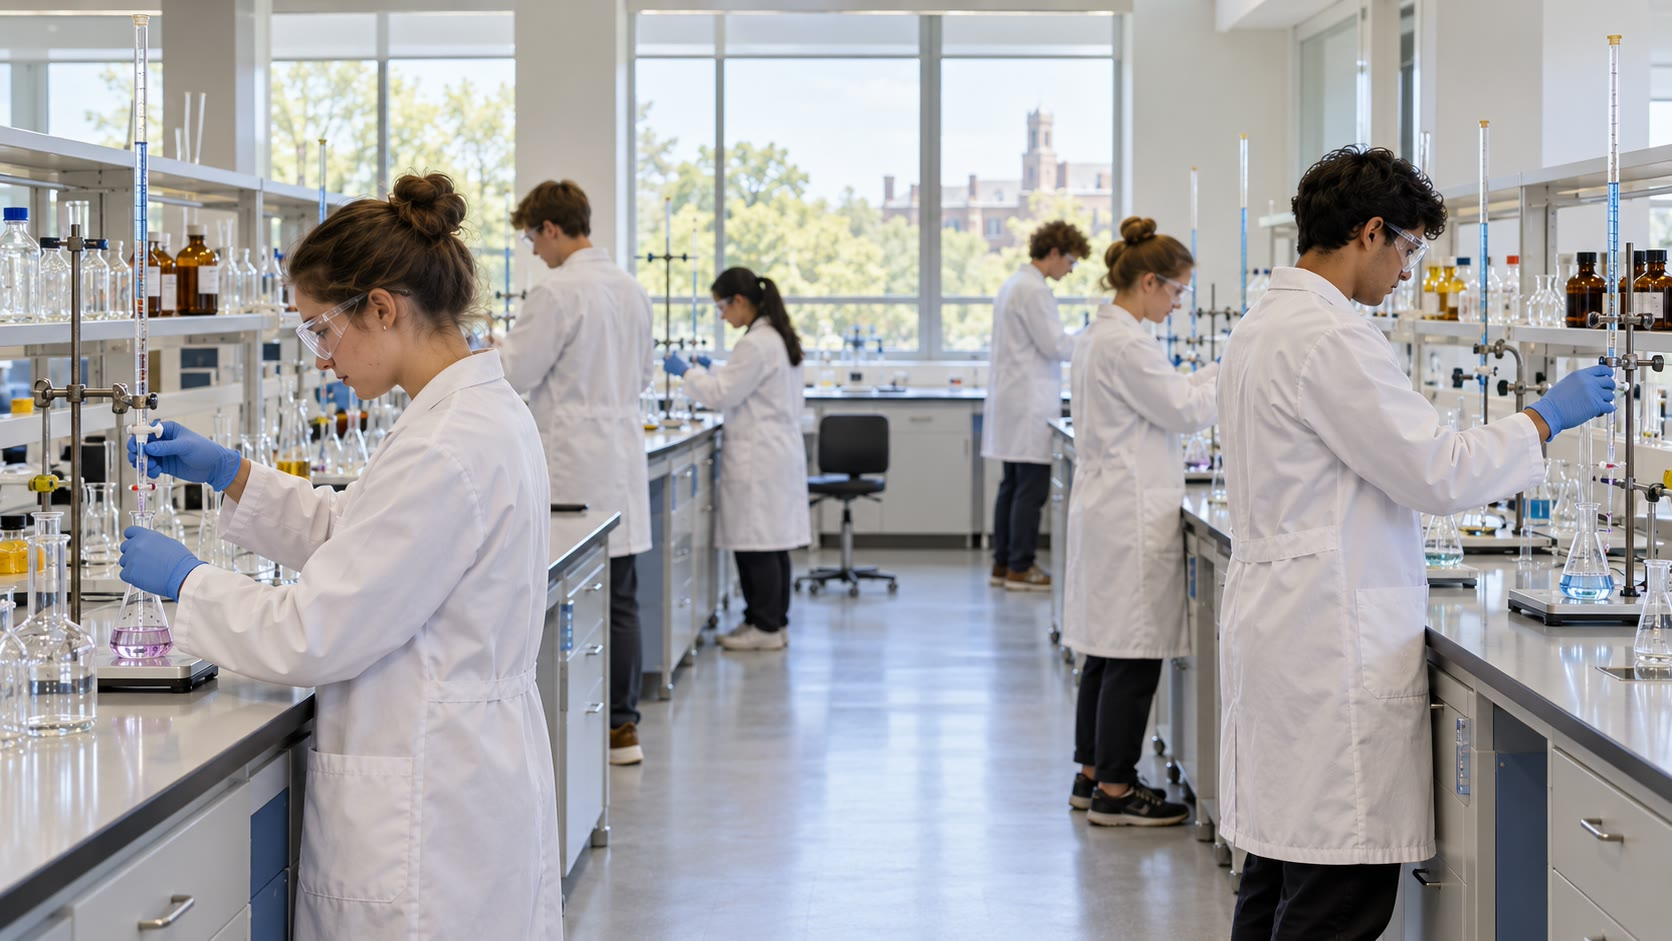
\includegraphics[width=0.66\linewidth]{images/book2/ai/b1-15-teaching-lab.jpg}

{\small Sebuah laboratorium pengajaran: buret, labu Erlenmeyer di atas
pengaduk magnetik, sarung tangan, dan kacamata pelindung. \omterm{def:b1:titration-methods:titration}{Titrasi} adalah
cara penetapan kadar yang paling umum dalam kimia.}
\end{omfigure}

\section{Titrasi dan ekuivalensi}

\begin{definition}[Titrasi, ekuivalensi]\label{def:b1:titration-methods:titration}
\emph{Titrasi}\index{titrasi} menentukan jumlah sebuah spesies, yaitu
\emph{analit}\index{analit}, melalui reaksi dengan pereaksi yang
konsentrasinya diketahui, yaitu \emph{titran}\index{titran}, yang
ditambahkan sedikit demi sedikit. Reaksinya harus tunggal, \omterm{def:b1:extent-q-and-k:quantitative}{kuantitatif}
($K$ besar), dan cepat. \emph{Ekuivalensi}\index{ekuivalensi} tercapai
ketika titran dan analit telah dipertemukan dalam perbandingan
stoikiometri reaksinya; volume yang ditambahkan pada saat itu adalah
volume ekuivalen, dan titik kurva titrasi pada volume itu adalah
\emph{titik ekuivalen}\index{titik ekuivalen}. Volume tempat
eksperimenter berhenti, karena melihat perubahan warna atau patahan
pada kurva, adalah \emph{titik akhir}\index{titik akhir}; metode yang
baik membuat titik akhir berimpit dengan ekuivalensi.
\end{definition}

\begin{proposition}[Hubungan ekuivalensi]\label{prop:b1:titration-methods:equivalence}
Untuk reaksi \omterm{def:b1:titration-methods:titration}{titrasi} $a\,\mathrm{A} + b\,\mathrm{B} \to \cdots$, dengan
\omterm{def:b1:titration-methods:titration}{analit} A ($n_A$ mol) dan \omterm{def:b1:titration-methods:titration}{titran} B pada konsentrasi $C_B$, volume
ekuivalennya memenuhi
\[
  \frac{n_A}{a} = \frac{C_B V_{\mathrm{eq}}}{b} .
\]
\end{proposition}

\begin{proof}
Misalkan $x$ \omterm{def:b1:extent-q-and-k:extent}{kemajuan reaksi} sesudah penambahan volume \omterm{def:b1:titration-methods:titration}{titran} $V$.
Sebelum \omterm{def:b1:titration-methods:titration}{ekuivalensi} B adalah \omterm{def:b1:extent-q-and-k:max-extent}{pereaksi pembatas} dan, karena reaksinya
\omterm{def:b1:extent-q-and-k:quantitative}{kuantitatif}, $x = C_BV/b$; sesudahnya, A adalah \omterm{def:b1:extent-q-and-k:max-extent}{pereaksi pembatas} dan
$x = n_A/a$. \omterm{def:b1:titration-methods:titration}{Ekuivalensi} adalah volume ketika keduanya habis bersamaan,
$n_A - ax = 0$ dan $C_BV - bx = 0$: dengan mengeliminasi $x$ diperoleh
hubungan itu.
\end{proof}

\section{Titrasi langsung dan tidak langsung}

\begin{definition}[Jenis-jenis titrasi]\label{def:b1:titration-methods:kinds}
Dalam \emph{titrasi langsung}\index{titrasi langsung}, \omterm{def:b1:titration-methods:titration}{titran} bereaksi
dengan \omterm{def:b1:titration-methods:titration}{analit} itu sendiri. Dalam
\emph{titrasi balik}\index{titrasi balik}, sejumlah pereaksi berlebih yang diketahui ditambahkan ke \omterm{def:b1:titration-methods:titration}{analit},
dan kelebihan yang tersisa dititrasi. Jika sebuah larutan mengandung
beberapa \omterm{def:b1:titration-methods:titration}{analit} yang bereaksi secara bergiliran dengan \omterm{def:b1:titration-methods:titration}{titran},
\omterm{def:b1:titration-methods:titration}{analit-analit} itu diukur melalui \emph{titrasi
berurutan}\index{titrasi berurutan}, satu \omterm{def:b1:titration-methods:titration}{ekuivalensi} demi satu
\omterm{def:b1:titration-methods:titration}{ekuivalensi}; jika semuanya bereaksi bersamaan dan memberikan satu
\omterm{def:b1:titration-methods:titration}{ekuivalensi} saja, melalui
\emph{titrasi simultan}\index{titrasi simultan}, yang hanya memberikan jumlah totalnya.
\end{definition}

\begin{method}[Titrasi balik]\label{met:b1:titration-methods:back-titration}
Gunakan \omterm{def:b1:titration-methods:kinds}{titrasi balik} jika reaksi langsungnya lambat, jika \omterm{def:b1:titration-methods:titration}{analitnya}
tidak stabil atau mudah menguap, atau jika tidak ada indikator yang cocok
untuk reaksi langsungnya.
\begin{enumerate}
  \item Tambahkan sejumlah $n_R$ pereaksi R yang diketahui, secara
        berlebih, dan biarkan bereaksi sempurna dengan \omterm{def:b1:titration-methods:titration}{analit} A
        ($\alpha\,\mathrm{A} + \rho\,\mathrm{R}$).
  \item Titrasilah kelebihan R dengan \omterm{def:b1:titration-methods:titration}{titran} T ($\rho'\,\mathrm{R} +
        \tau\,\mathrm{T}$) sampai volume ekuivalen $V_T$.
  \item Hitunglah $n_{R,\text{berlebih}} = \frac{\rho'}{\tau}C_TV_T$, lalu
        $n_A = \frac{\alpha}{\rho}(n_R - n_{R,\text{berlebih}})$.
\end{enumerate}
\end{method}

Soal akhir pekan mentitrasi vitamin C dengan cara ini: asam askorbat
mereduksi iodin yang berlebih, dan iodin yang tersisa dititrasi dengan
tiosulfat.

\section{Titrasi pH-metri dan indikator}

\begin{omfigure}
\begin{tikzpicture}[font=\small]
  \pic at (0,0) {stirrer};
  \pic at (0,0.18) {beaker={0.55}{omDef!14}};
  \pic at (0.2,2.45) {burette={0.75}{white}};
  \pic at (-0.45,0.45) {probe};
  \pic (m) at (-2.6,3.2) {meter={pH}};
  \draw[thick] (-0.45,3.45) to[out=90, in=0] (m-b);
  \node[anchor=west] at (0.65,6.2) {buret: NaOH, \qty{0.100}{mol/L}};
  \node[anchor=west] at (1.0,1.0) {asam, $V_0 = \qty{10.0}{mL}$, diencerkan};
  \draw[<-, omProp, thick] (1.2,-0.25) -- (1.8,-0.25) node[anchor=west, text=black] {pengaduk magnetik};
  \draw[<-, omProp, thick] (-0.62,2.4) -- (-1.5,2.0) node[anchor=east, text=black] {elektrode gabungan};
\end{tikzpicture}

{\small \omterm{def:b1:titration-methods:titration}{Titrasi} pH-metri. Elektrode kaca gabungan mengukur pH sesudah
setiap penambahan dari buret; pengaduk mencampur larutan. Elektrode itu
dikalibrasi terlebih dahulu dengan dua \omterm{def:b1:predominant-reaction:buffer}{larutan penyangga}.}
\end{omfigure}

\begin{omfigure}
\begin{tikzpicture}
\begin{axis}[name=s,
  width=0.5\linewidth, height=5.6cm, xmin=0, xmax=20, ymin=0, ymax=14,
  axis x line=bottom, axis y line=left, xlabel={$V$ (mL)}, ylabel={pH},
  xtick={0,5,10,15,20}, ytick={0,2,4,6,8,10,12,14},
  tick label style={font=\small}, label style={font=\small}]
\addplot[omDef, very thick] table[x=V, y=pH] {figdata/out/bachelor-1-titration-curves-strong.dat};
\addplot[omProp, thick] table[x=V, y=pH] {figdata/out/bachelor-1-titration-curves-weak.dat};
\node[font=\scriptsize, omDef, anchor=south west] at (axis cs:6,0.2) {\ce{HCl}};
\node[font=\scriptsize, omProp, anchor=west] at (axis cs:0.4,6.4) {\ce{CH3COOH}};
\draw[dotted] (axis cs:5,0) -- (axis cs:5,4.76) -- (axis cs:0,4.76);
\node[font=\scriptsize, anchor=north] at (axis cs:2.5,4.7) {$\mathrm{p}K_a$};
\end{axis}
\begin{axis}[at={(s.east)}, anchor=west, xshift=1.2cm,
  width=0.5\linewidth, height=5.6cm, xmin=0, xmax=20, ymin=0, ymax=14,
  axis x line=bottom, axis y line=left, xlabel={$V$ (mL)}, ylabel={pH},
  xtick={0,5,10,15,20}, ytick={0,2,4,6,8,10,12,14},
  tick label style={font=\small}, label style={font=\small}]
\addplot[omMeth, very thick] table[x=V, y=pH] {figdata/out/bachelor-1-titration-curves-mixture.dat};
\node[font=\scriptsize, anchor=west, align=left] at (axis cs:10.8,6.0) {\ce{HCl} + \ce{CH3COOH}\\ dua ekuivalensi};
\end{axis}
\end{tikzpicture}

{\small Kiri: \qty{10.0}{mL} asam klorida dan asam etanoat, keduanya
\qty{0.100}{mol/L}, yang dititrasi dengan natrium hidroksida
\qty{0.100}{mol/L}. \omterm{def:b1:predominant-reaction:strong-acid}{Asam lemah} mempunyai daerah penyangga dengan pH $=
\mathrm{p}K_a$ pada setengah \omterm{def:b1:titration-methods:titration}{ekuivalensi} dan \omterm{def:b1:titration-methods:titration}{titik ekuivalen} pada pH 8.73.
Kanan: sebuah campuran, masing-masing asam \qty{0.050}{mol/L}: \omterm{def:b1:predominant-reaction:strong-acid}{asam kuat}
dititrasi lebih dahulu (\omterm{def:b1:titration-methods:titration}{ekuivalensi} pada \qty{5}{mL}), lalu \omterm{def:b1:predominant-reaction:strong-acid}{asam lemah}
(\qty{10}{mL}).}
\end{omfigure}

\begin{proposition}[Setengah ekuivalensi asam lemah]\label{prop:b1:titration-methods:half-equivalence}
Jika \omterm{def:b1:predominant-reaction:strong-acid}{asam lemah} HA dititrasi dengan \omterm{def:b1:predominant-reaction:strong-acid}{basa kuat}, pada setengah \omterm{def:b1:titration-methods:titration}{ekuivalensi}
$\mathrm{pH} = \mathrm{p}K_a$, asalkan asamnya tidak terlalu kuat dan
tidak terlalu encer ($\mathrm{p}K_a$ kira-kira antara 4 dan 10 pada
\qty{0.1}{mol/L}).
\end{proposition}

\begin{proof}
Pada setengah \omterm{def:b1:titration-methods:titration}{ekuivalensi}, \omterm{def:b1:extent-q-and-k:quantitative}{reaksi kuantitatif} \ce{HA + OH- -> A- + H2O}
telah mengubah separuh HA: $[\mathrm{HA}] = [\mathrm{A^-}]$, dan hubungan
Henderson memberikan $\mathrm{pH} = \mathrm{p}K_a$. Syarat itu menjamin
bahwa reaksi HA dengan air dan reaksi $\mathrm{A^-}$ dengan air tidak
mengubah jumlah-jumlah itu secara berarti.
\end{proof}

\begin{proposition}[pH pada ekuivalensi asam lemah]\label{prop:b1:titration-methods:ph-at-equivalence}
Pada \omterm{def:b1:titration-methods:titration}{ekuivalensi} \omterm{def:b1:titration-methods:titration}{titrasi} \omterm{def:b1:predominant-reaction:strong-acid}{asam lemah} ($\mathrm{p}K_a$) dengan \omterm{def:b1:predominant-reaction:strong-acid}{basa kuat},
larutannya berupa basa konjugasi pada konsentrasi $C'$ (sesudah
pengenceran), dan
\[
  \mathrm{pH} = \tfrac12(\mathrm{p}K_e + \mathrm{p}K_a + \log C') .
\]
\end{proposition}

\begin{proof}
\omterm{def:b1:predominant-reaction:predominant-reaction}{Reaksi predominan} basa itu dengan air,
\ce{A- + H2O <=> HA + OH-}, mempunyai $K = K_e/K_a$; dengan sedikit basa
yang berubah, $[\ce{OH-}] = \sqrt{KC'}$ (\cref{prop:b1:predominant-reaction:ph-formulas}),
sehingga diperoleh hasil itu. Untuk asam etanoat, $C' = \qty{0.050}{mol/L}$:
$\frac12(14.00 + 4.76 - 1.30) = 8.73$.
\end{proof}

\begin{proposition}[Titrasi berurutan]\label{prop:b1:titration-methods:successive}
Dua asam yang dititrasi dengan basa yang sama memberikan \omterm{def:b1:titration-methods:titration}{ekuivalensi} yang
terpisah, masing-masing dengan ketelitian lebih baik daripada
\qty{1}{\percent}, jika $\mathrm{p}K_a$-nya berselisih sedikitnya 4.
\end{proposition}

\begin{proof}
Pada \omterm{def:b1:titration-methods:titration}{ekuivalensi} pertama, reaksi basa $\mathrm{A_1^-}$ dengan asam kedua
$\mathrm{HA_2}$, $\mathrm{A_1^-} + \mathrm{HA_2}
\rightleftharpoons \mathrm{HA_1} + \mathrm{A_2^-}$, mempunyai $K = 10^{\mathrm{p}K_1 - \mathrm{p}K_2}$.
Mulai dari jumlah yang sama, bagian $x$ asam kedua yang telah dititrasi
memenuhi $x^2/(1 - x)^2 = K$; untuk $x \leqslant 0.01$, $K
\leqslant 10^{-4}$, yaitu $\mathrm{p}K_2 - \mathrm{p}K_1 \geqslant 4$.
\end{proof}

Asam fosfat (2.15, 7.21, 12.34) memberikan dua \omterm{def:b1:titration-methods:titration}{ekuivalensi} yang jelas;
\omterm{def:b1:titration-methods:titration}{ekuivalensi} ketiga hilang dalam air basanya. Asam etanoat yang
bercampur dengan asam klorida (kanan gambar) dititrasi sesudahnya, karena
\omterm{def:b1:predominant-reaction:strong-acid}{asam kuat} itu pada hakikatnya ber-$\mathrm{p}K_a$ di bawah 0.

\begin{method}[Menentukan letak ekuivalensi pada kurva]\label{met:b1:titration-methods:derivative}
\begin{enumerate}
  \item Turunan: hitunglah $\Delta\mathrm{pH}/\Delta V$ antara
        titik-titik yang berurutan; \omterm{def:b1:titration-methods:titration}{ekuivalensi} terletak pada maksimumnya.
  \item Garis singgung: gambarlah dua garis singgung sejajar pada kurva di
        kedua sisi lonjakan, dan garis sejajar yang berjarak sama dari
        keduanya; garis itu memotong kurva di \omterm{def:b1:titration-methods:titration}{titik ekuivalen}.
\end{enumerate}
\end{method}

\begin{method}[Garis singgung, dengan perhitungan]\label{met:b1:titration-methods:tangents}
Untuk kurva yang direkam komputer, cocokkan titik-titik di setiap sisi
lonjakan dengan sebuah fungsi mulus dan ambillah titik beloknya; untuk
lonjakan yang simetris (\omterm{def:b1:predominant-reaction:strong-acid}{asam kuat}, \omterm{def:b1:predominant-reaction:strong-acid}{basa kuat}) titik tengah lonjakan pada
pH 7 adalah \omterm{def:b1:titration-methods:titration}{titik ekuivalennya}.
\end{method}

\begin{definition}[Indikator warna, trayek perubahan warna]\label{def:b1:titration-methods:indicator}
\emph{Indikator warna}\index{indikator warna} adalah \omterm{def:b1:predominant-reaction:bronsted}{pasangan asam--basa}
lemah HIn/In$^-$ yang kedua bentuknya berbeda warna. Warnanya berubah
pada \emph{trayek perubahan warna}\index{trayek perubahan warna}, yaitu
rentang pH tempat tidak ada bentuk yang jelas dominan, sekitar
$\mathrm{p}K_{a}(\mathrm{HIn}) \pm 1$.
\end{definition}

\begin{omfigure}
\begin{tabular}{lccl}
\hline
indikator & $\mathrm{p}K_a$ & trayek perubahan & warna (asam / basa) \\
\hline
jingga metil & 3.5 & 2.5--4.5 & merah / kuning \\
merah metil & 4.8 & 3.8--5.8 & merah / kuning \\
merah fenol & 7.9 & 6.9--8.9 & kuning / merah \\
biru timol (perubahan kedua) & 9.2 & 8.2--10.2 & kuning / biru \\
\hline
\end{tabular}

\smallskip
{\small Empat indikator, dengan $\mathrm{p}K_a$ dari kompilasi kritis
\omterm{def:b1:complexation:formation-constant}{tetapan disosiasi}; \omterm{def:b1:titration-methods:indicator}{trayek perubahan warnanya} $\mathrm{p}K_a \pm 1$.}
% ledger: pka:methylorange, pka:methylred, pka:phenolred, pka:thymolblue2
\end{omfigure}

\begin{method}[Memilih indikator]\label{met:b1:titration-methods:choose-indicator}
Pilihlah indikator yang \omterm{def:b1:titration-methods:indicator}{trayek perubahan warnanya} terletak di dalam
lonjakan tegak kurva, sedekat mungkin dengan pH pada \omterm{def:b1:titration-methods:titration}{ekuivalensi}. \omterm{def:b1:predominant-reaction:strong-acid}{Asam
kuat} dengan \omterm{def:b1:predominant-reaction:strong-acid}{basa kuat} (lonjakan 3.3 sampai 10.7 untuk
$\pm\qty{0.1}{mL}$ di sini): keempatnya. Asam etanoat (\omterm{def:b1:titration-methods:titration}{ekuivalensi} 8.73):
merah fenol atau biru timol; jingga metil akan berubah warna jauh
sebelum \omterm{def:b1:titration-methods:titration}{ekuivalensi}.
\end{method}

\section{Titrasi potensiometri}

\begin{definition}[Titrasi potensiometri]\label{def:b1:titration-methods:potentiometric}
\emph{Titrasi potensiometri}\index{titrasi potensiometri} mengikuti
potensial sebuah elektrode di dalam larutan terhadap \omterm{def:b1:nernst:reference-electrode}{elektrode acuan},
untuk \omterm{def:b1:titration-methods:titration}{titrasi} redoks (kawat platina), pengendapan (kawat perak), atau
kompleksasi.
\end{definition}

\begin{proposition}[Titik-titik istimewa titrasi redoks]\label{prop:b1:titration-methods:potentiometric-points}
Untuk \omterm{def:b1:titration-methods:titration}{titrasi} $\mathrm{Red_1}$ dengan $\mathrm{Ox_2}$ melalui
$n_2\,\mathrm{Red_1} + n_1\,\mathrm{Ox_2} \to n_2\,\mathrm{Ox_1} +
n_1\,\mathrm{Red_2}$ (pasangan dengan $n_1$ dan $n_2$ elektron), $E(V_{\mathrm{eq}}/2) = E^\circ_1$, $E(2V_{\mathrm{eq}}) =
E^\circ_2$, dan pada \omterm{def:b1:titration-methods:titration}{ekuivalensi}
\[
  E_{\mathrm{eq}} = \frac{n_1E^\circ_1 + n_2E^\circ_2}{n_1 + n_2},
\]
untuk pasangan-pasangan yang \omterm{def:b1:nernst:couple}{setengah reaksinya} tidak melibatkan spesies
lain (atau pada pH yang menjaga suku-suku tambahannya tetap).
\end{proposition}

\begin{proof}
Pada setengah \omterm{def:b1:titration-methods:titration}{ekuivalensi} separuh $\mathrm{Red_1}$ teroksidasi:
$[\mathrm{Ox_1}] = [\mathrm{Red_1}]$ dan \omterm{thm:b1:nernst:nernst}{persamaan Nernst} pasangan 1
memberikan $E^\circ_1$. Pada $2V_{\mathrm{eq}}$ jumlah $\mathrm{Ox_2}$
yang berlebih sama dengan yang telah tereduksi:
$[\mathrm{Ox_2}] = [\mathrm{Red_2}]$, $E = E^\circ_2$. Pada \omterm{def:b1:titration-methods:titration}{ekuivalensi},
kalikan \omterm{thm:b1:nernst:nernst}{persamaan Nernst} pasangan 1 dengan $n_1$ dan persamaan pasangan
2 dengan $n_2$, lalu jumlahkan; stoikiometrinya membuat
$[\mathrm{Ox_1}]/[\mathrm{Red_1}] \cdot [\mathrm{Ox_2}]/[\mathrm{Red_2}] = 1$
(jumlah $\mathrm{Red_1}$ dan $\mathrm{Ox_2}$ yang tersisa berbanding sama
dengan produk-produknya), sehingga logaritma-logaritmanya saling
meniadakan.
\end{proof}

Untuk besi(II) dengan permanganat dalam asam \qty{1}{mol/L}, $n_1 = 1$
dan $n_2 =
5$: $E_{\mathrm{eq}} = (0.77 + 5 \times 1.51)/6 = 1.39$~V. Lonjakannya,
dari sekitar 0.8 sampai 1.5~V, begitu besar sehingga \omterm{def:b1:titration-methods:titration}{titik akhirnya}
tajam; dalam praktik permanganat menjadi indikatornya sendiri, karena
warna ungunya bertahan pada tetes pertama yang berlebih.

\begin{omfigure}
\begin{tikzpicture}
\begin{axis}[name=p,
  width=0.5\linewidth, height=5.6cm, xmin=0, xmax=20, ymin=0.6, ymax=1.6,
  axis x line=bottom, axis y line=left, xlabel={$V$ (mL)}, ylabel={$E$ (V)},
  xtick={0,5,10,15,20},
  tick label style={font=\small}, label style={font=\small}]
\addplot[omDef, very thick] table[x=V, y=E] {figdata/out/bachelor-1-titration-curves-potentiometric.dat};
\draw[dotted] (axis cs:5,0.6) -- (axis cs:5,0.77) -- (axis cs:0,0.77);
\draw[dotted] (axis cs:10,0.6) -- (axis cs:10,1.39) -- (axis cs:0,1.39);
\node[font=\scriptsize, anchor=south west] at (axis cs:0.2,0.77) {0.77};
\node[font=\scriptsize, anchor=south west] at (axis cs:0.2,1.39) {1.39};
\end{axis}
\begin{axis}[at={(p.east)}, anchor=west, xshift=1.2cm,
  width=0.5\linewidth, height=5.6cm, xmin=0, xmax=20, ymin=0, ymax=4.6,
  axis x line=bottom, axis y line=left, xlabel={$V$ (mL)},
  ylabel={$\kappa$ (mS/cm)}, xtick={0,5,10,15,20},
  tick label style={font=\small}, label style={font=\small}]
\addplot[omProp, very thick] table[x=V, y=kappa] {figdata/out/bachelor-1-titration-curves-conductimetric.dat};
\draw[dotted] (axis cs:10,0) -- (axis cs:10,1.15);
\end{axis}
\end{tikzpicture}

{\small Kiri: \omterm{def:b1:titration-methods:potentiometric}{titrasi potensiometri} \qty{10.0}{mL} besi(II)
\qty{0.100}{mol/L} dengan permanganat \qty{0.0200}{mol/L} dalam asam
\qty{1}{mol/L} (elektrode platina, potensial terhadap elektrode
hidrogen). Kanan: \omterm{def:b1:titration-methods:titration}{titrasi} konduktometri \qty{100}{mL} asam klorida
\qty{0.0100}{mol/L} dengan natrium hidroksida \qty{0.100}{mol/L};
\omterm{def:b1:titration-methods:titration}{ekuivalensinya} terletak pada perpotongan dua garis lurus.}
% ledger: lam:H+, lam:OH-, lamsalt:HCl, lamsalt:NaCl (conductivities in figdata/bachelor-1/titration-curves.py)
\end{omfigure}

\section{Titrasi konduktometri, kompleksometri, dan pengendapan}

\begin{definition}[Konduktivitas ionik molar]\label{def:b1:titration-methods:conductivity}
Konduktivitas $\kappa$ sebuah larutan (dalam \unit{S/m}) mengukur
seberapa baik larutan itu menghantarkan arus melalui gerak ion-ionnya.
\emph{Konduktivitas ionik molar}\index{konduktivitas ionik molar}
$\lambda_i$ sebuah ion adalah sumbangannya per mol per satuan volume;
nilainya pada pengenceran tak berhingga, $\lambda_i^\circ$, adalah
tetapan ion itu dan pelarutnya pada suhu tertentu.
\end{definition}

\begin{proposition}[Hukum Kohlrausch]\label{prop:b1:titration-methods:kohlrausch}
Dalam larutan encer, konduktivitas adalah jumlah sumbangan ion-ionnya,
\[
  \kappa = \sum_i \lambda_i^\circ c_i ,
\]
yaitu \emph{hukum Kohlrausch}\index{hukum Kohlrausch}; konduktivitas
molar sebuah garam adalah jumlah konduktivitas molar ion-ionnya.
\end{proposition}

\admitted{\omterm{prop:b1:titration-methods:kohlrausch}{Hukum Kohlrausch} menyatakan bahwa ion-ion dalam larutan encer
bergerak secara bebas satu dari yang lain; batas-batasnya pada
konsentrasi yang lebih tinggi dipelajari dalam jilid Tahun~2. Di sini
hukum itu dipakai sebagai hukum eksperimen.}

\begin{proposition}[Kemiringan titrasi konduktometri]\label{prop:b1:titration-methods:conductimetric-slopes}
Jika \omterm{def:b1:predominant-reaction:strong-acid}{asam kuat} H$^+$X$^-$ dititrasi dengan \omterm{def:b1:predominant-reaction:strong-acid}{basa kuat} Na$^+$OH$^-$ dalam
volume yang besar (pengenceran diabaikan), konduktivitasnya berubah
secara linear terhadap volume yang ditambahkan, dengan kemiringan yang
sebanding dengan $\lambda^\circ(\ce{Na+}) - \lambda^\circ(\ce{H+}) < 0$
sebelum \omterm{def:b1:titration-methods:titration}{ekuivalensi} dan dengan
$\lambda^\circ(\ce{Na+}) + \lambda^\circ(\ce{OH-}) > 0$ sesudahnya.
\end{proposition}

\begin{proof}
Sebelum \omterm{def:b1:titration-methods:titration}{ekuivalensi} setiap mol hidroksida yang ditambahkan menghilangkan
satu mol \ce{H+} (\ce{H+ + OH- -> H2O}) dan membawa satu mol \ce{Na+};
sesudah \omterm{def:b1:titration-methods:titration}{ekuivalensi} hidroksida itu menambahkan satu \ce{Na+} dan satu
\ce{OH-}. \ce{X-} tidak berubah. Menurut \omterm{prop:b1:titration-methods:kohlrausch}{hukum Kohlrausch},
konduktivitasnya berubah sebesar gabungan $\lambda^\circ$ itu dikalikan
dengan jumlah yang ditambahkan dibagi dengan volume (yang tetap).
\end{proof}

Dari konduktivitas pembatas, $\lambda^\circ(\ce{H+}) =
\qty{349.8}{S.cm^2/mol}$ dan $\lambda^\circ(\ce{OH-}) = 198.3$, serta
konduktivitas garam \ce{HCl} (426) dan \ce{NaCl} (126.5), \omterm{prop:b1:titration-methods:kohlrausch}{hukum
Kohlrausch} memberikan
$\lambda^\circ(\ce{Cl-}) = 426 - 349.8 = 76.2$ dan $\lambda^\circ(\ce{Na+}) =
126.5 - 76.2 = 50.3$~\unit{S.cm^2/mol}. Ion hidrogen dan ion hidroksida
menghantarkan jauh lebih baik daripada ion-ion lainnya: kurvanya berupa
huruf V yang tajam.

\omterm{def:b1:titration-methods:titration}{Titrasi} kompleksometri memakai edta: pada pH 10 (penyangga amonia)
kalsium dan magnesium bereaksi dengannya secara \omterm{def:b1:extent-q-and-k:quantitative}{kuantitatif} (tetapan
kondisional pada \cref{ch:b1:complexation}), dan indikator yang juga
merupakan pengompleks lemah logam itu berubah warna ketika edta mengambil
ion-ion logam terakhir darinya --- \omterm{def:b1:titration-methods:titration}{titrasi} kesadahan air. \omterm{def:b1:titration-methods:titration}{Titrasi}
pengendapan memakai ion perak: klorida dititrasi dengan perak nitrat
dengan kromat sebagai indikator (\cref{exo:b1:precipitation:8}), atau
diikuti dengan elektrode perak (\cref{ch:b1:nernst}). Ketelitian semua
hasil ini, yang ditentukan oleh alat gelas dan \omterm{def:b1:titration-methods:titration}{titik akhirnya}, dibahas
pada \cref{ch:b1:lab-techniques-1}.

\section{Latihan}

\begin{exercise}[$\star$]\label{exo:b1:titration-methods:1}
\qty{20.0}{mL} larutan natrium hidroksida memerlukan \qty{12.4}{mL} asam
klorida \qty{0.100}{mol/L}. Tuliskan reaksinya beserta tetapannya, lalu
hitunglah konsentrasi basa itu.
\end{exercise}

\begin{exercise}[$\star$]\label{exo:b1:titration-methods:2}
Indikator manakah dalam tabel yang cocok untuk \omterm{def:b1:titration-methods:titration}{titrasi} amonia
(\qty{0.10}{mol/L}, $\mathrm{p}K_a = 9.25$) dengan asam klorida
\qty{0.10}{mol/L}? Hitunglah terlebih dahulu pH pada \omterm{def:b1:titration-methods:titration}{ekuivalensi}.
\end{exercise}

\begin{exercise}[$\star$]\label{exo:b1:titration-methods:3}
\qty{10.0}{mL} besi(II) dititrasi dengan permanganat \qty{0.0200}{mol/L};
warna ungu bertahan mulai \qty{12.6}{mL}. Tuliskan reaksinya dan
hitunglah konsentrasi besi(II).
\end{exercise}

\begin{exercise}[$\star$]\label{exo:b1:titration-methods:4}
Sampel air sebanyak \qty{50.0}{mL} dititrasi dengan edta
\qty{0.0100}{mol/L} pada pH 10; \omterm{def:b1:titration-methods:titration}{ekuivalensinya} pada \qty{14.2}{mL}. Edta
bereaksi satu banding satu dengan kalsium dan magnesium. Hitunglah
konsentrasi total kedua ion itu. Apakah ini \omterm{def:b1:titration-methods:kinds}{titrasi simultan} atau
\omterm{def:b1:titration-methods:kinds}{titrasi berurutan}?
\end{exercise}

\begin{exercise}[$\star\star$]\label{exo:b1:titration-methods:5}
Untuk \omterm{def:b1:titration-methods:titration}{titrasi} \qty{10.0}{mL} asam etanoat \qty{0.100}{mol/L} dengan
natrium hidroksida \qty{0.100}{mol/L}, hitunglah pH pada 0, 5.0, 10.0,
dan \qty{15.0}{mL} dengan metode-metode pada
\cref{ch:b1:predominant-reaction}, lalu bandingkan dengan kurva dalam
bab ini.
\end{exercise}

\begin{exercise}[$\star\star$]\label{exo:b1:titration-methods:6}
Tunjukkan bahwa \omterm{def:b1:titration-methods:titration}{titrasi} pH-metri asam fosfat dengan natrium hidroksida
memberikan dua lonjakan, lalu hitunglah pH pada setiap \omterm{def:b1:titration-methods:titration}{ekuivalensi} untuk
asam \qty{0.100}{mol/L} (\qty{10.0}{mL}, basa \qty{0.100}{mol/L}).
Mengapa tidak ada lonjakan ketiga?
\end{exercise}

\begin{exercise}[$\star\star$]\label{exo:b1:titration-methods:7}
Campuran asam klorida dan asam etanoat (\qty{10.0}{mL}) dititrasi dengan
natrium hidroksida \qty{0.100}{mol/L}: dua \omterm{def:b1:titration-methods:titration}{ekuivalensi}, pada
\qty{6.2}{mL} dan \qty{14.6}{mL}. Hitunglah kedua konsentrasinya. Berapa
pH di tengah-tengah antara kedua \omterm{def:b1:titration-methods:titration}{ekuivalensi} itu?
\end{exercise}

\begin{exercise}[$\star\star$]\label{exo:b1:titration-methods:8}
Hitunglah \omterm{def:b1:nernst:electrode-potential}{potensial elektrode} platina dalam \omterm{def:b1:titration-methods:titration}{titrasi} besi(II) dengan
permanganat (data dalam bab ini) pada 2.0, 9.0, 11.0, dan
\qty{20.0}{mL}.
\end{exercise}

\begin{exercise}[$\star\star$]\label{exo:b1:titration-methods:9}
Dengan \omterm{prop:b1:titration-methods:kohlrausch}{hukum Kohlrausch} dan nilai-nilai dalam bab ini, hitunglah
konduktivitas asam klorida yang dititrasi pada 0, 10.0, dan
\qty{20.0}{mL} basa (\qty{100}{mL} asam \qty{0.0100}{mol/L}, basa
\qty{0.100}{mol/L}, dengan memperhitungkan pengenceran), serta kedua
kemiringannya.
\end{exercise}

\begin{exercise}[$\star\star\star$]\label{exo:b1:titration-methods:10}
Buktikan bahwa kurva pH-metri \omterm{def:b1:predominant-reaction:strong-acid}{asam kuat} yang dititrasi dengan \omterm{def:b1:predominant-reaction:strong-acid}{basa kuat}
simetris terhadap \omterm{def:b1:titration-methods:titration}{titik ekuivalen} jika pengenceran diabaikan, lalu
hitunglah besar lonjakan antara $V_{\mathrm{eq}} \pm 0.1$~mL untuk \omterm{def:b1:titration-methods:titration}{titrasi}
dalam bab ini. Bagaimana lonjakan itu berubah jika semua konsentrasi
dibagi 100?
\end{exercise}

\begin{exercise}[$\star\star\star$]\label{exo:b1:titration-methods:11}
Turunkan persamaan kurva potensiometri besi(II) dengan permanganat
sebelum dan sesudah \omterm{def:b1:titration-methods:titration}{ekuivalensi}, lalu periksalah ketiga titik istimewa
pada \cref{prop:b1:titration-methods:potentiometric-points}. Bagaimana
potensial \omterm{def:b1:titration-methods:titration}{ekuivalensinya} berubah pada pH 1?
\end{exercise}

\begin{exercise}[$\star\star\star$]\label{exo:b1:titration-methods:12}
Amonium klorida (\qty{0.100}{mol/L}, $\mathrm{p}K_a = 9.25$) tidak dapat
dititrasi secara akurat dengan natrium hidroksida memakai indikator.
Jelaskan dari kurvanya, lalu usulkan sebuah \omterm{def:b1:titration-methods:kinds}{titrasi balik}: natrium
hidroksida berlebih, didihkan untuk mengusir amonia, lalu \omterm{def:b1:titration-methods:titration}{titrasi}
hidroksida yang tersisa dengan asam klorida. Tuliskan perhitungannya.
\end{exercise}

\section{Soal: Berapa Banyak Vitamin C dalam Tablet?}

\begin{problem}[{Soal akhir pekan --- reaksi iodin dengan asam askorbat,
titrasi balik dengan tiosulfat, perhitungan hasilnya, dan
ketidakpastiannya, diakhiri dengan massa asam askorbat per tablet}]
\label{pb:b1:titration-methods:1}
Sebuah tablet digerus dan dilarutkan dalam air di dalam labu ukur
\qty{100.0}{mL}. Sebuah alikuot \qty{10.00}{mL} diambil dengan pipet, lalu
ditambahkan \qty{20.00}{mL} larutan iodin \qty{0.0250}{mol/L} (berlebih).
Iodin yang tersisa dititrasi dengan natrium tiosulfat \qty{0.0500}{mol/L}
dengan amilum sebagai indikator: warna birunya hilang pada
\qty{8.90}{mL}. Asam askorbat adalah \ce{C6H8O6} ($M = \qty{176.0}{g/mol}$);
iodin mengoksidasinya menjadi \ce{C6H6O6}. $E^\circ(\ce{I2}/\ce{I-}) = 0.53$~V,
$E^\circ(\ce{S4O6^2-}/\ce{S2O3^2-}) = 0.02$~V.

\medskip
\noindent\textbf{Bagian I --- Reaksi-reaksinya.}
\begin{enumerate}
  \item Tuliskan \omterm{def:b1:nernst:couple}{setengah reaksi} pasangan \ce{C6H6O6}/\ce{C6H8O6}.
  \item Tuliskan reaksi iodin dengan asam askorbat.
  \item Tentukan \omterm{def:b1:nernst:oxidation-number}{bilangan oksidasi} iodin dalam \ce{I2} dan \ce{I-}.
  \item Tuliskan reaksi iodin dengan tiosulfat dan hitunglah tetapannya.
  \item Amilum memberikan warna biru pekat dengan iodin. Mengapa warna itu
        hilang tepat pada \omterm{def:b1:titration-methods:titration}{ekuivalensi} \omterm{def:b1:titration-methods:titration}{titrasi} tiosulfat?
  \item Asam askorbat perlahan-lahan dioksidasi oleh oksigen udara.
        Mengapa hal itu mendukung penambahan iodin sekaligus, secara
        berlebih?
\end{enumerate}

\medskip
\noindent\textbf{Bagian II --- Mengapa \omterm{def:b1:titration-methods:kinds}{titrasi balik}?}
\begin{enumerate}[resume]
  \item Apa yang diperlukan untuk \omterm{def:b1:titration-methods:kinds}{titrasi langsung} asam askorbat dengan
        iodin?
  \item Paparkan \omterm{def:b1:titration-methods:kinds}{titrasi balik} itu sebagai ketiga langkah pada
        \cref{met:b1:titration-methods:back-titration}.
  \item Mengapa iodin harus berlebih? Periksalah dengan hasilnya.
  \item Mengapa larutan tiosulfat dibakukan sesaat sebelum dipakai?
  \item Alikuotnya \qty{10.00}{mL} dari \qty{100.0}{mL}: berapa faktor
        pengencerannya?
  \item Alat gelas manakah yang mengalirkan \qty{20.00}{mL} larutan iodin
        itu?
\end{enumerate}

\medskip
\noindent\textbf{Bagian III --- Perhitungannya.}
\begin{enumerate}[resume]
  \item Hitunglah jumlah iodin yang dimasukkan.
  \item Hitunglah jumlah tiosulfat yang terpakai.
  \item Turunkan jumlah iodin yang berlebih.
  \item Turunkan jumlah iodin yang bereaksi dengan asam askorbat.
  \item Hitunglah jumlah asam askorbat dalam alikuot.
  \item Hitunglah jumlah, lalu massa, asam askorbat dalam tablet.
  \item Bandingkan dengan labelnya (\qty{500}{mg}).
\end{enumerate}

\medskip
\noindent\textbf{Bagian IV --- Seberapa yakin?}
Toleransinya: labu \qty{100.0 \pm 0.1}{mL}, pipet
\qty{10.00 \pm 0.02}{mL} dan \qty{20.00 \pm 0.03}{mL}, pembacaan buret
$\pm\qty{0.05}{mL}$; kedua konsentrasi diketahui sampai \qty{0.2}{\percent}.
\begin{enumerate}[resume]
  \item Nyatakan $n(\text{asam askorbat})$ dalam tablet sebagai fungsi
        besaran-besaran yang terukur.
  \item Ketidakpastian relatif manakah yang masuk ke dalam jumlah iodin
        yang dimasukkan dan jumlah yang berlebih?
  \item Mengapa selisih dua jumlah memperbesar ketidakpastian relatif?
  \item Dengan menggabungkan sumbangan-sumbangannya seperti pada
        \cref{ch:b1:lab-techniques-1} (jumlah kuadratis), perkirakan
        ketidakpastian relatif hasilnya.
  \item Tuliskan massa asam askorbat per tablet beserta
        ketidakpastiannya, sampai dua angka penting.
\end{enumerate}
\end{problem}
